\documentclass{article}

\usepackage[spanish]{babel}
\usepackage[numbers,sort&compress]{natbib}
\usepackage[T1]{fontenc}
\usepackage[ansinew]{inputenc}
\usepackage{graphicx}
\usepackage{url}
\usepackage{caption}
\usepackage{float}
\usepackage{subcaption}
\usepackage{caption}
\usepackage{listings}
\usepackage{amsmath}
\usepackage{natbib}
\usepackage[numbers,sort&compress]{natbib}

\title {B\'usqueda Local}
\author{Oscar Qui\~nonez}

\begin{document}

\maketitle
 
\section{Objetivo}\label{met}

Utilizando el m\'etodo heur\'istico se busca representar la posici\'on de un objeto mediante el uso de diferentes rutas, al encontrar la mas corta, conoceremos l\'ogicamente, la mas cercana, que ser\'a representada en una proyecci\'on tridimensional en forma de un mapa topogr\'afico.

\section{Metodolog\'ia}\label{met}

Partiendo del c\'odigo base \cite{satuelisa} proporcionado anteriormente en clase, se busca desarrollar la simulaci\'on mediante el uso del programa R 4.0.3, en el cual se variaron los valores entre los ejes $g(x,y)$, que van de $-3 \leq x, y \leq 3$, de esta forma hacer que se recorran las rutas con pasos de 1.5 hasta completar una ruta de 100 pasos.

\section{Resultados y Discusi\'on}\label{res}

Se obtuvo una gr\'afica que se muestra como figura 1, en la que se puede observar una notable diferencia con la figura 2, que fue la figura obtenida con el c\'odigo original ya antes mencionado, esta diferencia en la cantidad de intersecciones se debe a la aproximaci\'on al origen con respecto al n\'umero de repeticiones.
As\'i tambi\'en se observa una diferencia en los planos mostrados en las figuras 3 y 4, pues las intersecciones se dan en una menor cantidad de repeticiones y nos damos cuenta como se deshace la simetr\'ia de los planos. Todas las figuras estan disponibles \cite{yo} en el repositorio de la clase.
\begin{figure}
  \centering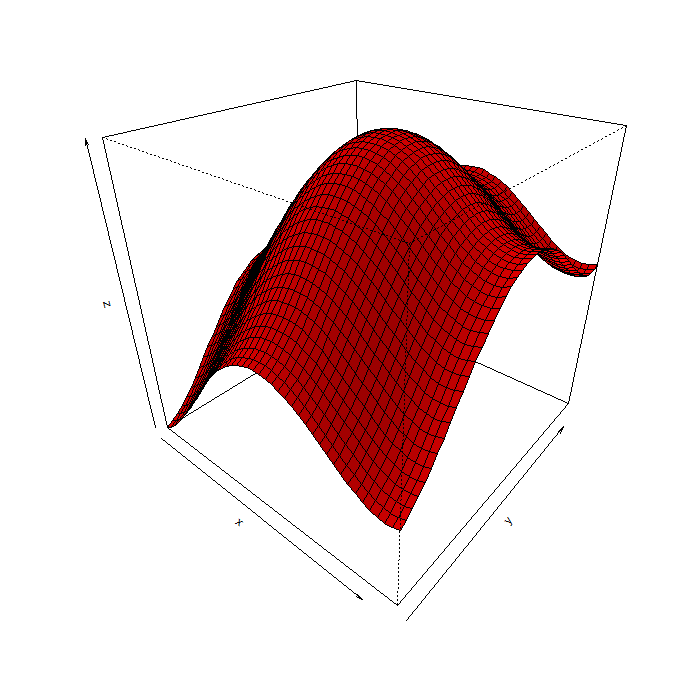
\includegraphics[scale=0.6]{tareasiete_2d.png}
  \caption{Gr\'afica con el c\'odigo modificado.}
  \label{fig}
\end{figure}

\begin{figure}
  \centering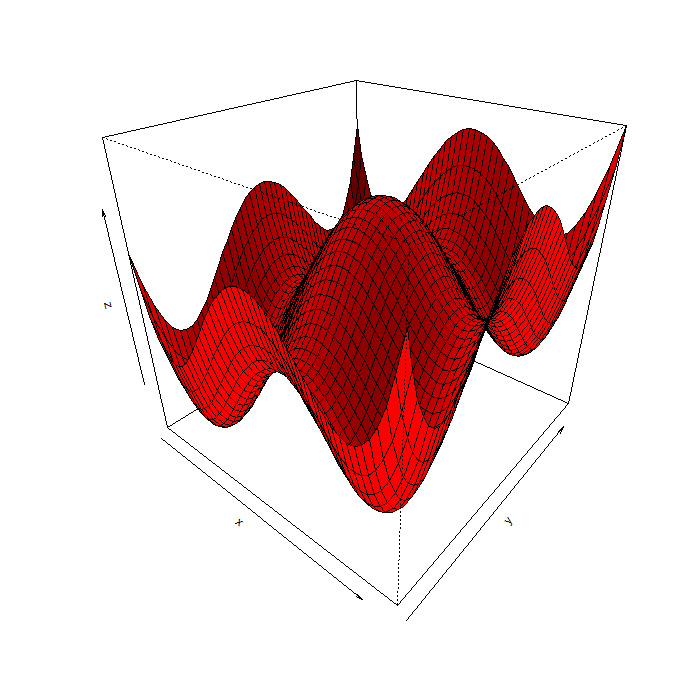
\includegraphics[scale=0.6]{1tareasiete_2d.png}
  \caption{Gr\'afica con el c\'odigo original.}
  \label{fig}
\end{figure}

\begin{figure}
       \centering
       \begin{subfigure}[b]{0.48\linewidth}
           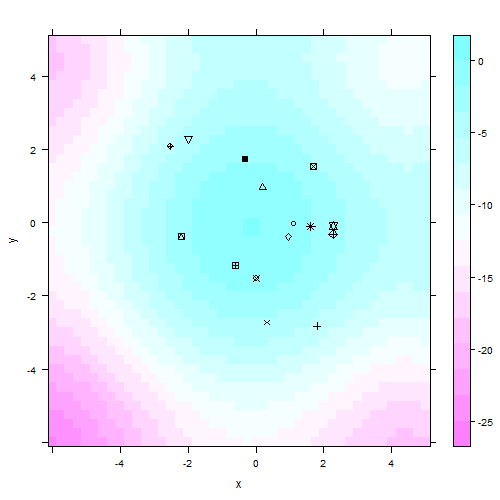
\includegraphics[width=\linewidth]{tarea7sim_1001.png}
           \caption{Inicial}
           \label{fig:westminster_lateral}
        \end{subfigure}
        \begin{subfigure}[b]{0.48\linewidth}
            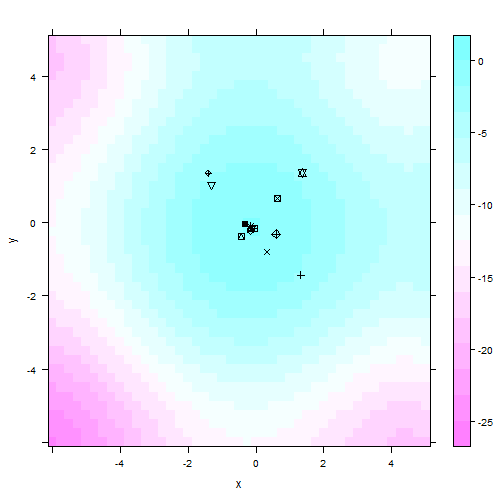
\includegraphics[width=\linewidth]{tarea7sim_1025.png}
            \caption{repetici\'on 25}
            \label{fig:westminster_aerea}
        \end{subfigure}
        \begin{subfigure}[b]{0.48\linewidth}
            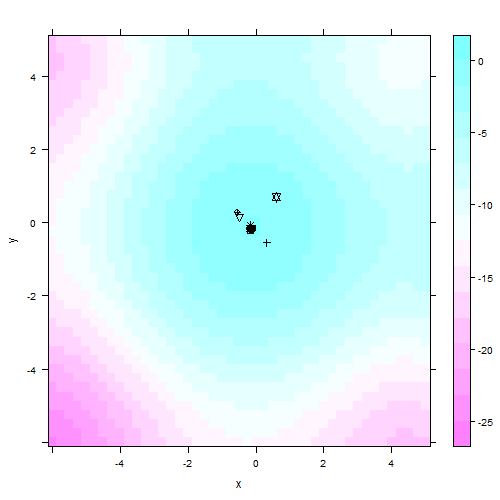
\includegraphics[width=\linewidth]{tarea7sim_1050.png}
            \caption{repetici\'on 50}
            \label{fig:westminster_aerea}
        \end{subfigure}
        \begin{subfigure}[b]{0.48\linewidth}
            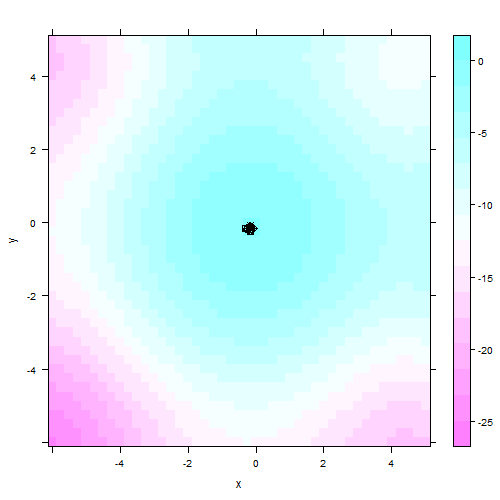
\includegraphics[width=\linewidth]{tarea7sim_1100.png}
            \caption{repetici\'on 100}
            \label{fig:westminster_aerea}
        \end{subfigure}
        \caption{Posici\'on inicial, repetici\'on 25, repetici\'on media 50 y repetici\'on final 100 (funci\'on mofificada $g(x, y)$).}
        \label{fig:westminster}
\end{figure}

\begin{figure}
       \centering
       \begin{subfigure}[b]{0.48\linewidth}
           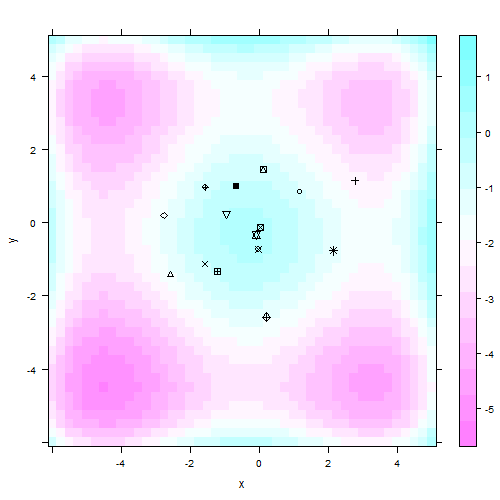
\includegraphics[width=\linewidth]{1tarea7sim_1001.png}
           \caption{Inicial}
           \label{fig:westminster_lateral}
        \end{subfigure}
        \begin{subfigure}[b]{0.48\linewidth}
            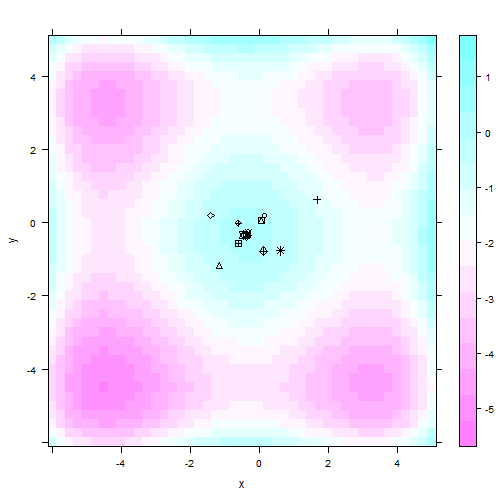
\includegraphics[width=\linewidth]{1tarea7sim_1025.png}
            \caption{repetici\'on 25}
            \label{fig:westminster_aerea}
        \end{subfigure}
        \begin{subfigure}[b]{0.48\linewidth}
            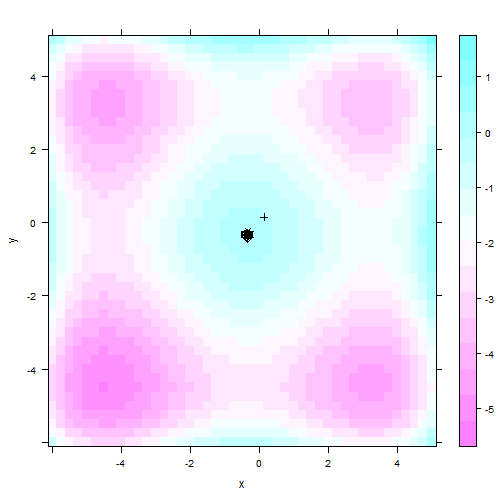
\includegraphics[width=\linewidth]{1tarea7sim_1050.png}
            \caption{repetici\'on 50}
            \label{fig:westminster_aerea}
        \end{subfigure}
        \begin{subfigure}[b]{0.48\linewidth}
            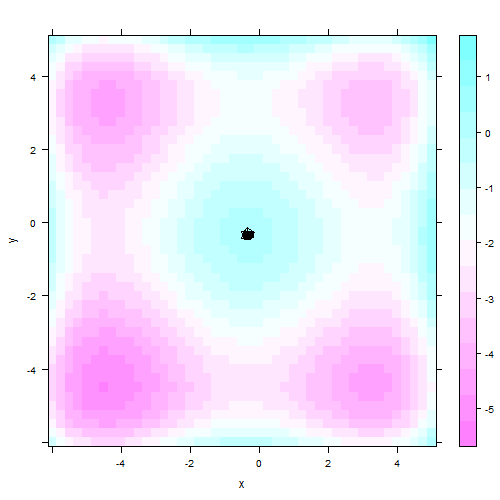
\includegraphics[width=\linewidth]{1tarea7sim_1100.png}
            \caption{repetici\'on 100}
            \label{fig:westminster_aerea}
        \end{subfigure}
        \caption{Posici\'on inicial, repetici\'on 25, repetici\'on media 50 y repetici\'on final 100 (funci\'on original $g(x, y)$).}
        \label{fig:westminster}
\end{figure}

\newpage
\section{Conclusi\'on}

Despu\'es de haber realizado la simulaci\'on se muestra que el m\'etodo heur\'istico nos ayuda a encontrar el camino mas corto en una simulaci\'on de una ruta pues como se vio en las gr\'aficas anteriores, el punto de intersecci\'on en el origen se encuentra de manera m\'as precisa, adem\'as como sabemos al modificar la funci\'on tambi\'en cambia la forma en la aproximaci\'on. 

\section{Reto 1}
En este reto se simula un tratamiento t\'ermico muy conocido, el recocido, este tratamiento se le da a los metales para cambiar su estructura interna y as\'i modificar sus propiedades, especialmente la dureza y maleabilidad. El par\'ametro que se busca modificar es la temperatura con valores entre 5 y 40 grados y as\'i vemos la influencia de esta en el valor de $\xi$. Como se aprecia en la figura 5, la variaci\'on es muy peque\~na y se determina que en este rango de temperaturas las propiedades no cambiar\'an mucho, pero probablemente lo hagan con temperaturas mas altas pues en 40 grados es donde comienza a verse una diferencia notable.
\begin{figure}
  \centering\includegraphics[scale=0.9]{reto1.png}
  \caption{Gr\'afica de caja-bigote para cada temperatura.}
  \label{fig}
\end{figure}
\newpage
\bibliography{tareasiete}
\bibliographystyle{unsrtnat}

\end{document}
